\documentclass[12pt, french]{article}

\usepackage{fancyhdr, fancybox, lastpage,mhchem, mathrsfs, tikz,amsfonts}
\usepackage[most]{tcolorbox}
\usepackage[a4paper, margin={0.3in, .75in}]{geometry}
\usepackage{wrapfig}
\pagestyle{fancy}
\renewcommand\headrulewidth{1pt}
\renewcommand\footrulewidth{1pt}
\fancyhf{}
\rhead{ \em{Zakaria Haouzan}}
\lhead[C]{\em{2ème année baccalauréat Sciences Physiques}}
\chead[C]{}
\rfoot[C]{}
\lfoot[R]{}
\cfoot[]{\em{Page \thepage / \pageref{LastPage}}}


\newtcolorbox{Box2}[2][
enhanced, 
    breakable,
]{
                lower separated=false,
                colback=white,
colframe=white!20!black,fonttitle=\bfseries,
colbacktitle=white!30!gray,
coltitle=black,
enhanced,
attach boxed title to top left={yshift=-0.1in,xshift=0.15in},
title=#2,#1}


\begin{document}
\begin{center}
   \shadowbox {\bf{ atome et mécanique de Newton }
 }

\end{center}
On utilisera les données suivantes :
$h = 6, 626 \times 10^{-34} J.s$; $c = 2, 998 \times 10^8 m/s$; $e = 1, 602 × 10^{-19}C$, $1eV = 1, 60 \times 10^{-19}J$
\vspace{-0.2cm}
%%_________________________Exercice ! :"_________________________Exercice
   \begin{Box2}{Exercice 1 : atome de lithium}

	   \begin{enumerate}
		   \item  L’atome de lithium $(Li)$, dans son premier état excité $(E_2 = 3, 54eV )$, émet une radiation de longueur d’onde $\lambda = 670, 3nm$ lorsqu’il se désexcite. En déduire l’énergie de l’état fondamental (en eV).

\item Le même atome, pour passer au niveau supérieur $E_3$ , doit absorber un photon de fréquence $\nu = 3, 69 \times 10^{14}Hz$.n Déterminer $E_3$ (en eV).
\end{enumerate}
   \end{Box2}


%%_________________________Exercice !2 :"_________________________Exercice
\begin{Box2}{Exercice 2 :émission et absorption }
   % \begin{wrapfigure}[1]{r}{0.32\textwidth}
  %\begin{center}
	  %\vspace{-0.6cm}
	%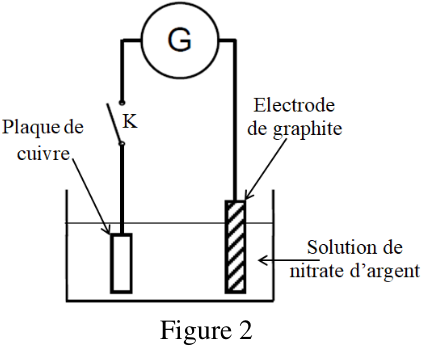
\includegraphics[width=0.32\textwidth]{./ex_01.png}
  %\end{center}
%\end{wrapfigure}

	\begin{enumerate}
		\item  Déterminer les longueurs d’onde émises par
la désexcitation de l’atome dont le diagramme
énergétique est celui ci- contre sachant que son
énergie initiale est $E_3$ .
Préciser le domaine auquel appartient chaque
rayonnement.
\item  On suppose, cette fois, que l’énergie de
l’atome ne peut excéder $E_3$ .
Quelles doivent être les longueurs d’onde de
photons incidents pour que l’atome puisse les
absorber ?
\end{enumerate}
  \begin{center}
	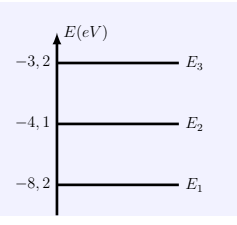
\includegraphics[width=0.3\textwidth]{./ex03.png}
  \end{center}



\end{Box2}

\begin{Box2}{Exercice 3 :ionisation }
	L’énergie d’un atome d’hydrogène au niveau n $(n \in \mathbb{N}^*)$ est :$$E_n = \frac{E_0}{n^2}$$
Avec $E_0 = 13, 6eV$ pour $_1^1H$  et $m(e^-) = 9, 11 \times 10^{-31}kg$.

\begin{enumerate}
	\item  Comment s’appelle le niveau $n = 1$ ? les niveaux correspondant à $n > 1$ ?
		
	\item  On considère que n varie de 1 à 8 (valeurs entières) ou que $n = \infty$. Expliquer succinctement pourquoi ce dernier état correspond à l’ionisation.

	\item  Calculer la longueur d’onde minimale d’un photon permettant d’ioniser l’atome d’hydrogène initialement dans son état     $n = 1$ (énergie de première ionisation). Refaire le même calcul pour n = 2.

		Calculer la vitesse de lélectron éjecté (en supposant que le noyau reste immobile).
	\item Exprimer l’énergie I de première ionisation d’un hydrogénoïde (atome ou ion à un seul électron, soit $_1H,_2He^{2+},_3Li^{2+}, ...)$ en fonction de $E_0$ et Z sachant que l’énergie d’un hydrogénoïde au niveau n est : $$E_n = \frac{E_0.Z^2}{n^2}$$
		où Z est le numéro atomique . et conclure.
		
\end{enumerate}


\end{Box2}
	%\vspace{-0.8cm}


%\begin{Box2}{Exercice 4 :Les toboggans}

%\end{Box2}




%\begin{Box2}{Exercice 5 : Etude du mouvement du centre de gravité d’une balle. }
%%\begin{wrapfigure}[3]{r}{0.33\textwidth}
	%%\vspace{-0.8cm}

%\end{Box2}


%\begin{center}
   %\Large{ \em{Exercices Supplémentaires}}
%\end{center}

%\vspace{-0.8cm}

%%%_________________________Exercice ! 3:"_________________________Exercice
%\begin{Box2}{Exercice 6:Etude du mouvement d’une balle de golf dans le champ de pesanteur uniforme }
%%\begin{wrapfigure}{r}{0.4\textwidth}
 %%\end{wrapfigure}

%\end{Box2}

%%_________________________Exercice 4 : _________________________Exercice
\begin{Box2}{Exercice 4 :Diagramme énergétique de l’atome d’hydrogène }
   %% \begin{wrapfigure}[12]{r}{0.5\textwidth}



Le document ci-contre est le diagramme
d’énergie de l’atome d’hydrogène .
Le niveau d’énergie le plus élevé $(n = \infty)$
correspond l’atome ionisé. On lui attribue ,
par convention , une énergie de valeur nulle .

Le niveau n=1 correspond à l’état fondamental .

Répondre par vrai ou faux aux propositions
suivantes en justifiant la réponse :
\begin{enumerate}
	\item  Les niveaux numérotés de $n=2$ à $n = \infty$
correspond à des états excités de l’atome .
\item  Le niveau d’énergie nulle est le plus stable.

\item  Lorsque l’atome passe du niveau $n=3$ à $n=2$ , il émet une radiation visible .

\item  Lorsque l’atome passe du niveau $n=1$ à
$n=3$ , il émet une radiation appartenant aux UV .
\item  Un atome d’hydrogène , pris dans son
état fondamental , peut absorber un photon
d’énergie $3,39Mev$ .
\end{enumerate}
  \begin{center}
	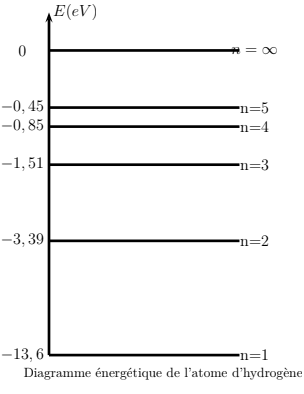
\includegraphics[width=0.3\textwidth]{./ex04.png}
  \end{center}


\end{Box2}


%\end{Box2}
\begin{center} \emph{\textbf{“The physical universe and its buzzing machinery, its fantastical scenery.”}}
\end{center}

%\vspace{-0.6cm}
%%%_________________________Exercice 5 : _________________________Exercice
%\begin{Box2}{Exercice 4 : }
   %% \begin{wrapfigure}[14]{r}{0.5\textwidth}
  %%\begin{center}
	  %%\vspace{-0.6cm}
	%%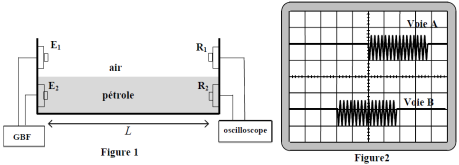
\includegraphics[width=0.5\textwidth]{./img/ex5.png}
  %%\end{center}
%%\end{wrapfigure}

%4

%\end{Box2}

%\begin{Box2}{Exercice 5 : }

%44
%\end{Box2}


%\begin{Box2}{Exercice 6 : }


	%\end{Box2}


%\begin{Box2}{Exercice 7 : }
%\end{Box2}
\end{document}
